\section{Definizione del prodotto}

% Nell'indice proposto da Tullio c'è:
% a. Metodo e formalismo di specifica
% b. Presentazione dell'architettura generale del sistema e identificazione dei componenti architetturali di alto livello

\subsection{Tecnologie utilizzate}
L'architettura è stata progettata cercando di tenere in considerazione diverse tecnologie, alcune delle quali espressamente richieste nel capitolato d'appalto. Vengono di seguito elencate e descritte le principali tecnologie impiegate e le motivazioni del loro utilizzo.

\begin{itemize}
	\item \textbf{Node.js} per contenere la logica lato server;
	\item \textbf{Express.js} come framework lato server: permette di sfruttare al massimo Node.js senza partire da zero;
	\item \textbf{MongoDB}: database di tipo NoSQL per la parte di recupero e salvataggio dei dati;
	\item \textbf{Mongoose} per l’interfacciamento con il database;
	\item \textbf{AngularJS} per l'interfaccia grafica: permette di usare il paradigma MVC anche in una pagina HTML.
\end{itemize}


\subsubsection{Node.js}
\textbf{Node.js} è un framework per realizzare applicazioni Web veloci e scalabili in JavaScript, permettendo di utilizzare questo linguaggio, tipicamente utilizzato nel lato client, anche per la scrittura di applicazioni lato server.
La piattaforma è basata su JavaScript Engine V8, che è il runtime di Google utilizzato anche da Chrome e disponibile sulle principali piattaforme. \newline
I principali vantaggi derivati dall'utilizzo di Node.js sono:
\begin{itemize}
	\item \textbf{Approccio asincrono}: Node.js permette di accedere alle risorse del sistema operativo in modalità event-driven e non sfruttando il classico modello basato su processi o thread concorrenti, utilizzato dai classici web server. Ciò garantisce una maggiore efficienza in termini di prestazioni poiché durante le attese, il runtime può gestire qualcos’altro in maniera asincrona.
	\item \textbf{Architettura modulare}: Lavorando con Node.js è molto facile organizzare il lavoro in librerie, importare i moduli e combinarli fra loro. In questo modo è possibile creare un applicazione scalabile e riproporzionata in base alle esigenze.
\end{itemize}

\subsubsection{Express.js}
\textbf{Express.js} è un framework per creare applicazioni Web con Node.js.
Mette a disposizione numerosi strumenti per realizzare rapidamente interfacce per la programmazione utilizzando il pattern MVC in modo semplice e veloce. Richiede moduli Node di terze parti per applicazioni che prevedono l’interazione con la basi di dati; \newline
\`E stato utilizzato il framework Express.js per supportare lo sviluppo dell'application server grazie alle utili e robuste features da esso offerte, le quali non mascherano alcuna funzionalità fornita da Node.js aprendo così le porte all'utilizzo di moduli per Node.js atti a supportare specifiche
funzionalità.

\subsubsection{MongoDB}
\textbf{MongoDB} è un database NoSQL open-source scalabile e altamente performante di tipo document-oriented, ovvero in cui i dati sono archiviati sotto forma di documenti in stile JSON con schema dinamici, secondo una struttura molto semplice e potente;
I principali vantaggi derivati dal suo utilizzo sono:
\begin{itemize}
	\item \textbf{Alte performance}: non ci sono join che possono rallentare le operazioni di lettura o scrittura; l’indicizzazione include gli indici di chiave anche sui documenti innestati e sugli array permettendo una rapida interrogazione al database;
	\item \textbf{Affidabilità}: alto meccanismo di replicazione su server;
	\item \textbf{Schemaless}: non esiste nessuno schema, è più flessibile e può essere facilmente trasformato in oggetti.	
	\item Permette di definire query complesse utilizzando un linguaggio che non è SQL;
	\item Permette di processare parallelamente i dati (Map-Reduce)
	\item Tipi di dato più flessibili.
\end{itemize}

\subsubsection{Mongoose}
\textbf{Mongoose} è una libreria per MongoDB che ci permette di definire degli schemi per modellare i dati del database, facendo rispettare una certa struttura ai dati per la creazione di nuovi Document. Inoltre fornisce molti strumenti utili per la validazione dei dati, per la definizione di query e per il casting dei tipi predefiniti. \newline
Per interfacciare l'application server con MongoDB sono disponibili diversi progetti open-source ed in questo caso è stato scelto di utilizzare Mongoose, attualmente il più diffuso.	

\subsection{Formalismo di specifica}

\subsection{Architettura di sistema}

\begin{figure}
\centering
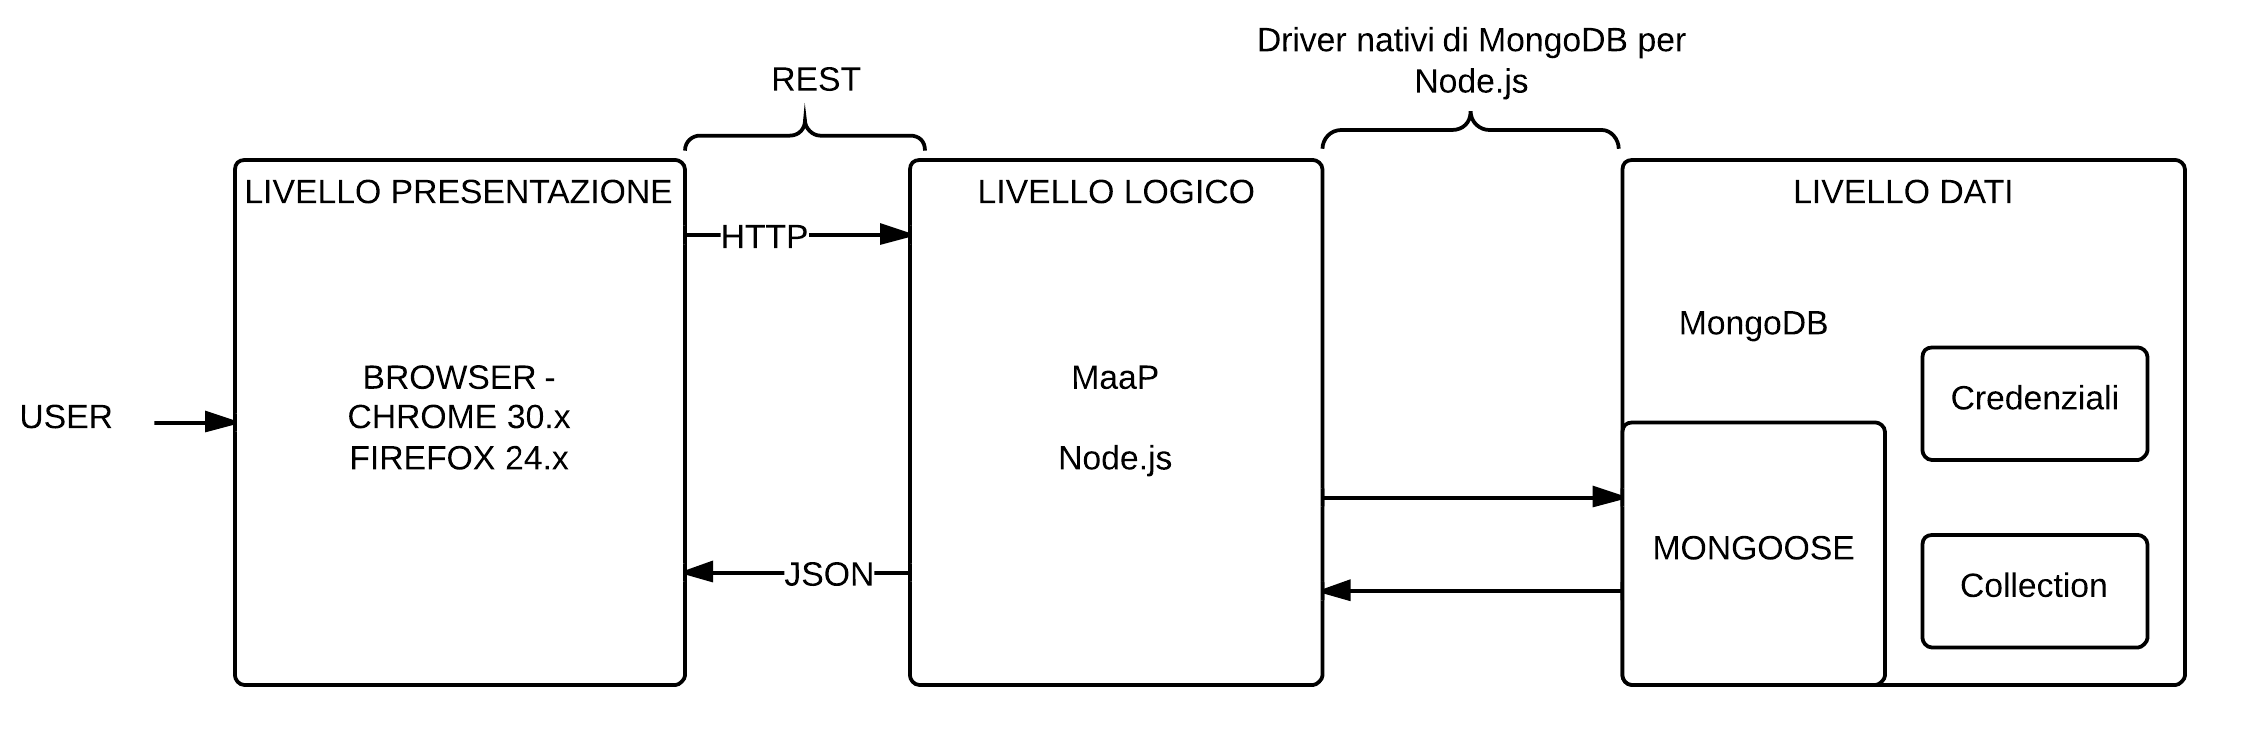
\includegraphics[scale=7]{3-TIER.png}
\caption{Schema del modello utilizzato}\label{fig:1}
\end{figure}

\subsection{Three-Tier Architecture}

Nota: Di seguito i termini modulo, strato e livello sono utilizzati .... 
Si tratta di un architettura di tipo client-server, in cui i processi logici, la persistenza dei dati e l'interfaccia utente sono sviluppati e mantenuti in moduli tra loro indipendenti e distribuiti, il vantaggio che ne consegue è che un modulo può essere aggiornato o sostituito senza dover alterare gli altri.
I tre livelli presenti sono:
\begin{itemize}
\item \textbf{Livello di presentazione} Si tratta dello strato che comunica con l'utente, il quale è estraneo all'esistenza degli altri moduli. Il compito di questo strato è fornire un'interfaccia utente, che comunicherà con il modulo logico per aggiornarsi e trasmettere le scelte dell'utente. Solitamente questo livello si trova sul client.
\item \textbf{Livello logico} Questo livello racchiude le funzionalità, i processi e gli algoritmi dell'applicazione. Solitamente questo livello si trova su un server, e si rapporta con il livello interfaccia e il livello dati. 
\item \textbf{Livello dati} In questo livello solitamente si trovano le \glossario{basi di dati} che garantiscono la persistenza dei dati. E' accessibili solo attraverso il livello logico, che ne garantisce la consistenza. In questo livello si trovano anche i componenti utili all'accesso della base di dati, nel nostro caso \glossario{Mongoose}.
E' importante far notare che uno strato dati può comunicare con più strati logici, che potranno utilizzare i dati in maniera diversa.
\end{itemize}


\subsubsection{REST}

REST, ovvero Representational State Transfer è un tipo di \glossario{RPC}. Si basa su un protocollo di comunicazione \glossario{stateless} di tipo client-server, e solitamente tale protocollo è \glossario{HTTP}, per \ProjectName è invece stato scelto \glossario{HTTPS}.

I motivi che hanno spinto alla scelta di REST sono:
\begin{itemize}
\item Semplicità di utilizzo;
\item Indipendenza dal sistema operativo utilizzato dal client;
\item Indipendente dai linguaggi di programmazione utilizzati;
\item In coppia con HTTPS permette una certa sicurezza delle comunicazioni.
\end{itemize}

REST utilizza il concetto di risorsa, ovvero un aggregato di dati con un nome (\glossario{URI}) e una rappresentazione, su cui è possibile invocare le operazioni \glossario{CRUD} tramite il protocollo sopracitato.

Nell'URL inviato sono presenti il nome della risorsa e la sua rappresentazione, identificata dall'estensione del file scelta, e per \ProjectName è stato scelto il formato \glossario{JSON}, in quanto il suo parsing in \glossario{JavaScript} è più semplice rispetto, ad esempio, quello di \glossario{XML} o \glossario{CSV}.

Un'altra caratteristica di REST è che essendo \glossario{stateless} ogni richiesta dovrà contenere tutte le informazioni necessarie, e non dipende dallo stato del sistema.
